%%%%%%%%%%%%  Generated using docx2latex.com  %%%%%%%%%%%%%%

%%%%%%%%%%%%  v2.0.0-beta  %%%%%%%%%%%%%%

% This template is made using Docx2Latex add-on for Google
% Docs, Do not request Edit Access instead make your 
% own copy using File > make a copy then navigate to 
% Add-ons > Docx2Latex > install/start to 
% use it. It will generate 100% perfect output according to
% guidelines of PICT TE-Seminar report guidelines.
\documentclass[12pt]{article}


 %%%%%%%%%%%%  Include Packages  %%%%%%%%%%%%%%


\usepackage{txfonts}
\usepackage{fancyhdr}
\fancypagestyle{plain}{%
 \fancyhf{}
 \fancyfoot[CE]{Pune Institute of Computer Technology, Department of Computer Engineering 2017-18}
 \fancyfoot[RE]{\thepage}
}
\pagestyle{fancy}
\fancyhead{}
\renewcommand{\headrulewidth}{0pt}
\footskip = 0.625in
\cfoot{}
\rfoot{}
% Blank space below is for aesthetics purpose only
\usepackage{amsmath}
\usepackage{latexsym}
\usepackage{amsfonts}
\usepackage[normalem]{ulem}
\usepackage{array}
\usepackage{amssymb}
\usepackage{graphicx}
\usepackage{subfig}
\usepackage{wrapfig}
\usepackage{wasysym}
\usepackage{enumitem}
\usepackage{adjustbox}
\usepackage{ragged2e}
\usepackage[svgnames,table]{xcolor}
\usepackage{tikz}
\usepackage{longtable}
\usepackage{changepage}
\usepackage{setspace}
\usepackage{hhline}
\usepackage{multicol}
\usepackage{tabto}
\usepackage{float}
\usepackage{multirow}
\usepackage{makecell}
\usepackage[toc,page]{appendix}
\usepackage[paperheight=11.69in,paperwidth=8.27in,left=1.0in,right=1.0in,top=1.0in,bottom=1.0in,headheight=1in]{geometry}
\usepackage[utf8]{inputenc}
\usepackage[T1]{fontenc}
\usepackage[hidelinks]{hyperref}
\usetikzlibrary{shapes.symbols,shapes.geometric,shadows,arrows.meta}
\tikzset{>={Latex[width=1.5mm,length=2mm]}}
\usepackage{flowchart}\TabPositions{0.5in,1.0in,1.5in,2.0in,2.5in,3.0in,3.5in,4.0in,4.5in,5.0in,5.5in,6.0in,}

\urlstyle{same}


 %%%%%%%%%%%%  Set Depths for Sections  %%%%%%%%%%%%%%

% 1) Section
% 1.1) SubSection
% 1.1.1) SubSubSection
% 1.1.1.1) Paragraph
% 1.1.1.1.1) Subparagraph


\setcounter{tocdepth}{5}
\setcounter{secnumdepth}{5}


 %%%%%%%%%%%%  Set Depths for Nested Lists created by \begin{enumerate}  %%%%%%%%%%%%%%


\setlistdepth{9}
\renewlist{enumerate}{enumerate}{9}
	\setlist[enumerate,1]{label=\arabic*)}
	\setlist[enumerate,2]{label=\alph*)}
	\setlist[enumerate,3]{label=(\roman*)}
	\setlist[enumerate,4]{label=(\arabic*)}
	\setlist[enumerate,5]{label=(\Alph*)}
	\setlist[enumerate,6]{label=(\Roman*)}
	\setlist[enumerate,7]{label=\arabic*}
	\setlist[enumerate,8]{label=\alph*}
	\setlist[enumerate,9]{label=\roman*}

\renewlist{itemize}{itemize}{9}
	\setlist[itemize]{label=$\cdot$}
	\setlist[itemize,1]{label=\textbullet}
	\setlist[itemize,2]{label=$\circ$}
	\setlist[itemize,3]{label=$\ast$}
	\setlist[itemize,4]{label=$\dagger$}
	\setlist[itemize,5]{label=$\triangleright$}
	\setlist[itemize,6]{label=$\bigstar$}
	\setlist[itemize,7]{label=$\blacklozenge$}
	\setlist[itemize,8]{label=$\prime$}

\setlength{\topsep}{0pt}\setlength{\parindent}{0pt}

 %%%%%%%%%%%%  This sets linespacing (verticle gap between Lines) Default=1 %%%%%%%%%%%%%%


\renewcommand{\arraystretch}{1.3}


%%%%%%%%%%%%%%%%%%%% Document code starts here %%%%%%%%%%%%%%%%%%%%



\begin{document}

\vspace{\baselineskip}

\vspace{\baselineskip}
\begin{Center}
{\fontsize{14pt}{16.8pt}\selectfont \textbf{PUNE INSTITUTE OF COMPUTER TECHNOLOGY,}\par}
\end{Center}\par

\begin{Center}
{\fontsize{14pt}{16.8pt}\selectfont \textbf{DHANKAWADI PUNE-43.}\par}
\end{Center}\par

\begin{Center}
{\fontsize{26pt}{31.2pt}\selectfont \textbf{\textit{A Seminar Report}}\par}
\end{Center}\par

\begin{Center}
\textbf{\textit{ }\ \ \ \  }{\fontsize{24pt}{28.8pt}\selectfont \textbf{\textit{\ On  }\  }\par}
\end{Center}\par

\begin{Center}
{\fontsize{16pt}{19.2pt}\selectfont \textbf{ Twitter Sentiment Analysis on}\par}
\end{Center}\par

\begin{Center}
{\fontsize{16pt}{19.2pt}\selectfont \textbf{Tourism using Lexicon Based Approach}\par}
\end{Center}\par

\begin{Center}
{\fontsize{14pt}{16.8pt}\selectfont  \par}
\end{Center}\par

\begin{Center}
{\fontsize{14pt}{16.8pt}\selectfont SUBMITTED BY\par}
\end{Center}\par

\begin{Center}
{\fontsize{14pt}{16.8pt}\selectfont  \par}
\end{Center}\par

\begin{Center}
{\fontsize{16pt}{19.2pt}\selectfont \textbf{NAME: Vikas Kodag}\par}
\end{Center}\par

\begin{Center}
{\fontsize{16pt}{19.2pt}\selectfont \textbf{ROLL NO: 3373}\par}
\end{Center}\par

\begin{Center}
{\fontsize{16pt}{19.2pt}\selectfont \textbf{CLASS: TE-3}\par}
\end{Center}\par

\begin{Center}
{\fontsize{7pt}{8.4pt}\selectfont \textbf{ }\par}
\end{Center}\par

\begin{Center}
{\fontsize{14pt}{16.8pt}\selectfont GUIDED BY\par}
\end{Center}\par

\begin{Center}
{\fontsize{16pt}{19.2pt}\selectfont \textbf{PROF. M. S. Takalikar}\par}
\end{Center}\par



%%%%%%%%%%%%%%%%%%%% Figure/Image No: 1 starts here %%%%%%%%%%%%%%%%%%%%

\begin{figure}[H]
	\begin{Center}
		\includegraphics[width=1.57in,height=1.57in]{image6.jpg}
	\end{Center}
\end{figure}


%%%%%%%%%%%%%%%%%%%% Figure/Image No: 1 Ends here %%%%%%%%%%%%%%%%%%%%

\begin{adjustwidth}{1.0in}{0.0in}
\begin{justify}
\ \ \ \ \ \ \ \ \ \ \ \ \ \ \ \ \ \  
\end{justify}\par

\end{adjustwidth}

 \par

 \par

 \par

\begin{Center}
{\fontsize{20pt}{24.0pt}\selectfont \textbf{COMPUTER ENGINEERING DEPARTMENT}\par}
\end{Center}\par

\begin{Center}
{\fontsize{20pt}{24.0pt}\selectfont \textbf{Academic Year: 2017-18}\par}

 %%%%%%%%%%%%  Starting New Page here %%%%%%%%%%%%%%

\newpage

\end{Center}\par


\vspace{\baselineskip}
\begin{Center}
{\fontsize{20pt}{24.0pt}\selectfont \textbf{ }\par}
\end{Center}\par

\begin{Center}
{\fontsize{14pt}{16.8pt}\selectfont \textbf{PUNE INSTITUTE OF COMPUTER TECHNOLOGY,}\par}
\end{Center}\par

\begin{Center}
{\fontsize{14pt}{16.8pt}\selectfont \textbf{DHANKAWADI PUNE-43.}\par}
\end{Center}\par


\vspace{\baselineskip}
\begin{Center}
{\fontsize{26pt}{31.2pt}\selectfont \textbf{\textit{CERTIFICATE}}{\fontsize{14pt}{16.8pt}\selectfont  \par}\par}
\end{Center}\par



%%%%%%%%%%%%%%%%%%%% Figure/Image No: 2 starts here %%%%%%%%%%%%%%%%%%%%

\begin{figure}[H]
	\begin{Center}
		\includegraphics[width=1.57in,height=1.57in]{image6.jpg}
	\end{Center}
\end{figure}


%%%%%%%%%%%%%%%%%%%% Figure/Image No: 2 Ends here %%%%%%%%%%%%%%%%%%%%

\begin{justify}
{\fontsize{14pt}{16.8pt}\selectfont \ \ \ \ \ \ \ \ \ \ \ \ \ \ \ \ \ \ \ \ \ \ \ \ \ \ \ \ \ \ \ \ \ \ \ \ \ \ \ \ \ \ \ \ \  \par}
\end{justify}\par

\begin{justify}
{\fontsize{18pt}{21.6pt}\selectfont This is to certify that {\fontsize{20pt}{24.0pt}\selectfont Mr.\textit{ \textbf{\uline{Vikas Kodag}} }{\fontsize{18pt}{21.6pt}\selectfont \textit{, R}oll No\textbf{. }{\fontsize{20pt}{24.0pt}\selectfont \textbf{\uline{3373}}{\fontsize{18pt}{21.6pt}\selectfont \uline{ }a student of T.E. (Computer Engineering Department) Batch 2017-2018, has satisfactorily completed a seminar report on $``${\fontsize{16pt}{19.2pt}\selectfont \textbf{ Twitter Sentiment Analysis on Tourism using Lexicon Based Approach$"$ }{\fontsize{18pt}{21.6pt}\selectfont  under the guidance of \uline{Prof. M. S. Takalikar} towards the partial fulfillment of the third year Computer Engineering Semester II of Pune University.\par}\par}\par}\par}\par}\par}\par}
\end{justify}\par

\begin{justify}
{\fontsize{18pt}{21.6pt}\selectfont  \par}
\end{justify}\par


\vspace{\baselineskip}


%%%%%%%%%%%%%%%%%%%% Table No: 1 starts here %%%%%%%%%%%%%%%%%%%%


\begin{table}[H]
 			\centering
\begin{tabular}{p{2.94in}p{2.94in}}
\hline
%row no:1
\multicolumn{1}{p{2.94in}}{Prof. M. S. Takalikar } & 
\multicolumn{1}{p{2.94in}}{\Centering Dr.\ R.B.Ingle  } \\
\hhline{~~}
%row no:2
\multicolumn{1}{p{2.94in}}{\textbf{Internal Guide}\textit{\  }} & 
\multicolumn{1}{p{2.94in}}{\Centering \textbf{Head of Department\textit{,}}} \\
\hhline{~~}
%row no:3
\multicolumn{1}{p{2.94in}}{} & 
\multicolumn{1}{p{2.94in}}{\Centering \textbf{Computer Engineering} } \\
\hhline{~~}

\end{tabular}
 \end{table}


%%%%%%%%%%%%%%%%%%%% Table No: 1 ends here %%%%%%%%%%%%%%%%%%%%


\vspace{\baselineskip}
\setlength{\parskip}{6.0pt}
{\fontsize{14pt}{16.8pt}\selectfont \textbf{Date:}\par}\par

{\fontsize{14pt}{16.8pt}\selectfont \textbf{Place:}\par}

 %%%%%%%%%%%%  Starting New Page here %%%%%%%%%%%%%%

\newpage
\par

\begin{Center}
{\fontsize{14pt}{16.8pt}\selectfont \textbf{ }\par}
\end{Center}\par

\begin{Center}
{\fontsize{16pt}{19.2pt}\selectfont \textbf{Twitter Sentiment Analysis on}\par}
\end{Center}\par

\begin{Center}
{\fontsize{16pt}{19.2pt}\selectfont \textbf{Tourism Using Lexicon Based Approach}\par}
\end{Center}\par

\begin{Center}
{\fontsize{14pt}{16.8pt}\selectfont \textbf{ }\par}
\end{Center}\par

 \par


% Following code generates Table Of Contents
% List Of Figures
% and Table Of Tables
\tableofcontents
\listoffigures
\listoftables
 \par

\begin{justify}
{\fontsize{14pt}{16.8pt}\selectfont \textbf{\textit{ }}\par}
\end{justify}\par


\newpage



\begin{justify}
{\fontsize{14pt}{16.8pt}\selectfont \textbf{\textit{Abstract:}}\par}
\end{justify}\par

\begin{justify}
\textit{\textcolor[HTML]{00000A}{Sentimental Analysis is reference to the task of Natural Language Processing to determine whether a text contains subjective information and what information it expresses i.e., whether the attitude behind the text is positive, negative or neutral. It is also known as emotion extraction or opinion mining. This is a very popular field of research in text mining. The basic idea is to find the polarity of the text and classify it into positive, negative or neutral. It helps in human decision making. To perform sentiment analysis, one has to perform various tasks like subjectivity detection, sentiment classification, aspect term extraction, feature extraction etc.}}
\end{justify}\par


\vspace{\baselineskip}
\begin{justify}
{\fontsize{14pt}{16.8pt}\selectfont \textbf{\textit{Keywords}}\textit{:} \textit{\textcolor[HTML]{00000A}{Sentiment Analysis, Opinion Mining, Social Networks, Classifiers, Supervised learning, Unsupervised learning.}}\par}
\end{justify}\par


\newpage


 %%%%%%%%%%%%  Starting New Page here %%%%%%%%%%%%%%

\newpage

\vspace{\baselineskip}\section*{ 1\hspace*{10pt}INTRODUCTION}
\addcontentsline{toc}{section}{ 1\hspace*{10pt}INTRODUCTION}
\begin{justify}
Sentiment Analysis (also referred as opinion mining) is the study of affective states and subjective information in the customer data (such as reviews and survey responses, online and social media) by using natural language processing and data mining techniques [1]. Sentiment analysis aims to determine the attitude of a subject with respect to some topic or the overall contextual polarity or emotional reaction to some object, such as a document, interaction, or event. The attitude may be a judgment or evaluation, affective state, or the intended emotional communication.
\end{justify}\par

\begin{justify}
For opinion mining or sentiment analysis some methods are applied like – Naive Bayes Machine Learning Classifier, Sentiwordnet, Support Vector Machine. Here we have used Lexicon based approach of Sentiment Analysis.Sentiment lexicon is used in the lexicon based approach. Sentiment lexicon is a collection of known and defined words. A specific sentiment is assigned to each word in the collection. The lexicon based approach is divided into dictionary based approach and corpus based approach[2].
\end{justify}\par

\begin{justify}
Sentiment analysis task is divided into three categories; Aspect level, Sentence level, Document level [3]. Aspect level analysis deal with the aspects of items. It can also be considered as phrase level analysis. In Sentence level, each sentence is considered as an entity. Summation method is used to provide overall result of the document. In document level, the whole document is considered as a single entity.
\end{justify}\par


\vspace{\baselineskip}

\newpage

\vspace{\baselineskip}

\vspace{\baselineskip}

\vspace{\baselineskip}

\vspace{\baselineskip}

\vspace{\baselineskip}

\vspace{\baselineskip}

\vspace{\baselineskip}

\vspace{\baselineskip}

\vspace{\baselineskip}

\vspace{\baselineskip}

\vspace{\baselineskip}

\vspace{\baselineskip}
\subsection*{1.1\hspace*{10pt}Motivation}
\addcontentsline{toc}{subsection}{1.1\hspace*{10pt}Motivation}
\begin{justify}
Twitter Sentiment Analysis was thoroughly dealt by Alec Go, Richa Bhayani and Lei Huang, Computer Science graduate students of Stanford University. They used various classifiers, including Naive Bayes, Maximum Entropy as well as Support Vector Machines to classify the tweets. The feature extractors used by them were both unigrams and bigrams combined. Parts of speech tag was used because same word may have different meaning depending on its usage. The data-set used by them was huge, comprising 1.6 million tweets divided equally into positive and negative classes.
\end{justify}\par

\begin{justify}
We have chosen to work with twitter since we feel it is a better approximation of public sentiment as opposed to conventional internet articles and web blogs. The reason is that the amount of relevant data is much larger for twitter, as compared to traditional blogging sites. Moreover the response on twitter is more prompt and also more general (since the number of users who tweet is substantially more than those who write web blogs on a daily basis). Sentiment analysis of public is highly critical in macro-scale phenomena like predicting the needs of tourist and their opinions on the tourism spot. This could be done by analysing overall public sentiment towards the place with respect to time for finding the correlation between public sentiment and the place of interest. The government can also estimate the changes to be made, facilities to be provided to attract more tourists in the future and in which a negative response was registered since twitter allows us to download stream of geo-tagged tweets for particular locations. Other applications of Sentiment Analysis includes the review of movies and products, popularity of an event. Predicting the results of popular political elections and polls is also an emerging application to sentiment analysis. One such study was conducted by Tumasjan et al. in Germany for predicting the outcome of federal elections in which concluded that twitter is a good reflection of offline sentiment 
\end{justify}\par


\vspace{\baselineskip}

\newpage

\vspace{\baselineskip}

\vspace{\baselineskip}

\vspace{\baselineskip}

\vspace{\baselineskip}

\vspace{\baselineskip}
\subsection*{1.2\hspace*{10pt}Literature Survey:}
\addcontentsline{toc}{subsection}{1.2\hspace*{10pt}Literature Survey:}
\begin{justify}
Sentiment analysis has been studied in wide area of domain such as movie review, teaching review [4], product review, e-learning, hotel review and many more. A small number of studies have focused on applying machine learning techniques in the tourism sector. 
\end{justify}\par


\vspace{\baselineskip}
\begin{justify}
A study [5] aimed to create a system that would assist users in understanding tourism opinions on the web by finding and extracting subjective information from reviews in tourism websites. Aspect extraction was performed with the use of frequent nouns and the opinion was determined. 
\end{justify}\par


\vspace{\baselineskip}
\begin{justify}
Estela Marine-Roig et al.[6] addressed the problem of finding out the frequently occurring trends of different tourist places from tourist opinions. The authors proposed a trends extraction framework that consisted of five phases i.e. semi automatic downloading, arranging, cleaning, debugging, and analyzing. Trends extraction framework is better than previous method Liu (2011) in trends extraction because two extra phases of cleaning and debugging has been added up to eliminate the noise present in the tourist's opinions. The limitations of the work are that i. Method does not classify the derived frequent trends into positive and negative trends ii. method extracts same trend in one opinion sentence multiple times that create the reputation of trends iii. Method extracts many irrelevant and meaningless trends during classification. 
\end{justify}\par


\vspace{\baselineskip}
\begin{justify}
In another way to enhance the performance of opinion sentences extraction Shimada, K.. [7] used support vector machine for sentences classification. The authors addressed the problem to identify whether tweet on-site are more likelihood or tweet off-site. The authors proposed a method to evaluate on-site likelihood. Firstly, this method takes tweets and identifies tourism related tweets. Secondly, extracts tourism related tweets and deletes the remaining ones. Lastly classifies the extracted tweets on the basis of different features of tourist places using SVM. The finding of this paper is that classification has improved by applying the method of on-site likelihood filtering method. The same fact is shown in the results i.e. without applying this filtering method Recall=58.2$\%$  and Precision = 75.0$\%$  and after applying the filtering method Recall=65.0$\%$  and Precision=80.5$\%$ . If there is a location name at the start of any tweet then it is high onsite likelihood tweet. The limitations of the work are that i. mostly the comments of authors on tweets are more than any other person which are mostly positive or negative that create nose in sentiment analysis ii. method extracts some sentences in which no opinion about targeted tourist place is given that creates noise during classification of reviews.  
\end{justify}\par


\newpage

\vspace{\baselineskip}

\vspace{\baselineskip}
\subsection*{1.3\hspace*{10pt}Applications}
\addcontentsline{toc}{subsection}{1.3\hspace*{10pt}Applications}
\subsubsection*{1.3.1\hspace*{10pt}Support in decision making:}
\addcontentsline{toc}{subsubsection}{1.3.1\hspace*{10pt}Support in decision making:}
\begin{justify}
Decision making is a very important field of our life. Opinions extracted from reviews helps us in making various decisions like $``$which books to buy$"$ , $``$which hotel to go$"$ , $``$which movie to watch$"$  etc.
\end{justify}\par

\subsubsection*{1.3.2\hspace*{10pt}Business application:}
\addcontentsline{toc}{subsubsection}{1.3.2\hspace*{10pt}Business application:}
\begin{justify}
In today’s world of competition, every company wants to satisfy its customers requirements by creating new innovative products. Assessments of individuals are an essential angle today with the goal that organizations can get an input from clients and can roll out sought improvements in their item. Google Product Search is one illustration.
\end{justify}\par

\subsubsection*{1.3.3\hspace*{10pt}Predictions and trend analysis:}
\addcontentsline{toc}{subsubsection}{1.3.3\hspace*{10pt}Predictions and trend analysis:}
\begin{justify}
Sentiment analysis enables one to predict market trends by tracking views of public. It is also helpful in elections where candidates wants to know the expectations of people from them. It is also used to follow the events that are trending right now.
\end{justify}\par


\vspace{\baselineskip}

\newpage

\vspace{\baselineskip}

\vspace{\baselineskip}

\vspace{\baselineskip}

\vspace{\baselineskip}

\vspace{\baselineskip}

\vspace{\baselineskip}

\vspace{\baselineskip}

\vspace{\baselineskip}

\vspace{\baselineskip}

\vspace{\baselineskip}

\vspace{\baselineskip}

\vspace{\baselineskip}

\section*{2\hspace*{10pt}PROPOSED MATHEMATICAL MODEL}
\addcontentsline{toc}{section}{2\hspace*{10pt}PROPOSED MATHEMATICAL MODEL}
\textcolor[HTML]{00000A}{Let S be the set which defines the system.}\par

\textcolor[HTML]{00000A}{S = $ \{ $ s, e, X, Y, Fm, DD, NDD, Su, Fl$ \} $ }\par

\textcolor[HTML]{00000A}{s = Start State}\par

\textcolor[HTML]{00000A}{e = End State}\par

\textcolor[HTML]{00000A}{X = Input Set = $ \{ $ Manually annotated sentiments, Input sentence$ \} $ }\par

\textcolor[HTML]{00000A}{Y = Output Set = $ \{ $ Polarity of the input sentence$ \} $ }\par

\textcolor[HTML]{00000A}{Fm = Set of functions = $ \{ $ F1, F2, F3$ \} $ }\par

\textcolor[HTML]{00000A}{Where,}\par

\textcolor[HTML]{00000A}{F1() = $ \{ $ Tokenizing the input sentences into words$ \} $ }\par

\textcolor[HTML]{00000A}{F2() = $ \{ $ classifies sentence as subjective and objective$ \} $ }\par

\textcolor[HTML]{00000A}{F3() = $ \{ $ Determines the polarity of the sentence along with polarity value and normalized\tab  value$ \} $ }\par

\textcolor[HTML]{00000A}{\ \ \ \ \ \ \ \ \ \ \ \ \ \ \ \ \ \ \ \ \ \ \ \ \ \ \ \ \ \ \ \ \ \ \ \ \ \ \ \ \ \ \ \ \ \ \ \ \ \ \ \ \ \ \ \ \ \ \ \ \ \ \ \ \  \tab }\par

\textcolor[HTML]{00000A}{DD = Deterministic Data}\par

\textcolor[HTML]{00000A}{ \tab  = $ \{ $ X$ \} $ }\par

\textcolor[HTML]{00000A}{NDD = Non-Deterministic Data}\par

\textcolor[HTML]{00000A}{ \tab \ \ \  = $ \{ $ Y$ \} $ }\par

\textcolor[HTML]{00000A}{Su= Success case =$ \{ $  Sentiment got classified according to the correct polarity $ \} $ }\par

\textcolor[HTML]{00000A}{Fl=Failure case=$ \{ $  Polarity of the sentence is reversed $ \} $ }\par

\begin{justify}
{\fontsize{15pt}{18.0pt}\selectfont \textbf{ }\par}
\end{justify}\par

\setlength{\parskip}{12.0pt}
\begin{justify}
\textbf{ }
\end{justify}\par

\section*{3\hspace*{10pt}DESIGN AND ANALYSIS OF SYSTEM}
\addcontentsline{toc}{section}{3\hspace*{10pt}DESIGN AND ANALYSIS OF SYSTEM}
\subsection*{3.1  Process Pipeline}
\addcontentsline{toc}{subsection}{3.1  Process Pipeline}
\begin{Center}


%%%%%%%%%%%%%%%%%%%% Figure/Image No: 3 starts here %%%%%%%%%%%%%%%%%%%%

\begin{figure}[H]
	\begin{Center}
		\includegraphics[width=6.56in,height=3.36in]{image8.png}
		\caption{Process Pipeline}
		\label{fig:Process Pipeline}
	\end{Center}
\end{figure}


%%%%%%%%%%%%%%%%%%%% Figure/Image No: 3 Ends here %%%%%%%%%%%%%%%%%%%%

\\
\textbf{\textit{}}
\end{Center}\par


\vspace{\baselineskip}
The current pipeline that is implemented in sentiment.py is depicted in the following diagram. Initially, the input text is split into sentences and each sentence is fed to a high precision subjectivity classifier. If the sentence is classified as subjective then syntactic patterns are learned from this instance. In case that the sentence is not detected as such then it is fed to the pattern-based classifier. The pattern-based classifier outputs the class of the sentence based on the learned patterns so far. If the instance is subjective then again more patterns are learned from it, otherwise it is fed to a high precision objectivity classifier. If the sentence is classified as objective, then it is ignored, otherwise it is fed to the polarity classifier. Finally, the polarity classifier estimates the numerical sentiment and normalized sentiment values and outputs the result.\par

\subsection*{3.2\  Subjective Classifier}
\addcontentsline{toc}{subsection}{3.2\  Subjective Classifier}
The high precision subjectivity classifiers are used to classify the sentences as $``$Subjective$"$ . The high-precision classifiers use lists of lexical items. Many of the subjective clues are from manually developed resources. The subjectivity clues are divided into those that are strongly subjective and those that are weakly subjective, using a combination of manual review and empirical results. A strongly subjective clue is one that is seldom used without a subjective meaning, whereas a weakly subjective clue is one that commonly has both subjective and objective uses.\par

The high-precision subjective classifier classifies a sentence as subjective if it contains two or more of the strongly subjective clues.\par

\subsection*{3.3 Objective Classifier}
\addcontentsline{toc}{subsection}{3.3 Objective Classifier}
The high-precision objective classifier takes a different approach. Rather than looking for the presence of lexical items, it looks for their absence. It classifies a sentence as objective if there are no strongly subjective clues and at most one weakly subjective clue in the current, previous, and next sentence combined.\par

The similar approach for objectivity classification is not taken as the sentences containing objective clues does not readily lead to high precision objective classification. Add sarcasm or a negative evaluation to a sentence about a dry topic such as stock prices, and the sentence becomes subjective. Conversely, add objective topics to a sentence containing two strongly subjective words such as odious and scumbag, and the sentence remains subjective.\par


\vspace{\baselineskip}
The bootstrapping process for subjective and objective classifier is given below\par


\vspace{\baselineskip}
\begin{Center}


%%%%%%%%%%%%%%%%%%%% Figure/Image No: 4 starts here %%%%%%%%%%%%%%%%%%%%

\begin{figure}[H]
	\begin{Center}
		
\includegraphics[width=6.27in,height=3.33in]{image11.png}
		\caption{Bootstrapping Process}
		\label{fig:Bootstrapping Process}
	\end{Center}
\end{figure}


%%%%%%%%%%%%%%%%%%%% Figure/Image No: 4 Ends here %%%%%%%%%%%%%%%%%%%%

\\
\textbf{}
\end{Center}\par

\subsection*{3.4\ \ \  Polarity Classifier}
\addcontentsline{toc}{subsection}{3.4\ \ \  Polarity Classifier}
A two-step approach was adopted to contextual polarity disambiguation. For the first step, we concentrate on whether clue instances are neutral or polar in context (where polar in context refers to having a contextual polarity that is positive, negative or both). For the second step, we take all clue instances marked as polar in step one, and focus on identifying their contextual polarity.\par


\vspace{\baselineskip}
The three polarity features(modifies polarity, modified by polarity, conj polarity) look in a window of four words before, searching for the presence of particular types of polarity influencers. General polarity shifters reverse polarity (e.g., little truth, little threat). Negative polarity shifters typically make the polarity of an expression negative (e.g., lack of understanding). Positive polarity shifters typically make the polarity of an expression positive (e.g., abate the damage).\par

\section*{4\hspace*{10pt}DISCUSSION ON IMPLEMENTATION RESULTS}
\addcontentsline{toc}{section}{4\hspace*{10pt}DISCUSSION ON IMPLEMENTATION RESULTS}
The proposed system was applied to the tweets gathered from twitter account of $``$GujratTourism$"$ . The final result are displayed in  Table \ref{tab:Results from Twitter Sentiment Analysis}.\par



%%%%%%%%%%%%%%%%%%%% Table No: 2 starts here %%%%%%%%%%%%%%%%%%%%


\begin{table}[H]
 			\centering
\begin{tabular}{p{1.45in}p{0.59in}}
\hline
%row no:1
\multicolumn{1}{|p{1.45in}}{\Centering Positive Sentiments} & 
\multicolumn{1}{|p{0.59in}|}{\Centering 681} \\
\hhline{--}
%row no:2
\multicolumn{1}{|p{1.45in}}{\Centering Negative Sentiments} & 
\multicolumn{1}{|p{0.59in}|}{\Centering 50} \\
\hhline{--}
%row no:3
\multicolumn{1}{|p{1.45in}}{\Centering Neutral Sentiments } & 
\multicolumn{1}{|p{0.59in}|}{\Centering 259} \\
\hhline{--}

\end{tabular}\caption{Results from Twitter Sentiment Analysis}
\label{tab:Results from Twitter Sentiment Analysis}

 \end{table}


%%%%%%%%%%%%%%%%%%%% Table No: 2 ends here %%%%%%%%%%%%%%%%%%%%

\setlength{\parskip}{0.0pt}
\begin{Center}

\end{Center}\par


\vspace{\baselineskip}
The system was also tested against random dataset comprising of 420 manually annotated sentences. The results are displayed in  Table \ref{tab:Sentiment Analysis on Random Sentences}.\par



%%%%%%%%%%%%%%%%%%%% Table No: 3 starts here %%%%%%%%%%%%%%%%%%%%


\begin{table}[H]
 			\centering
\begin{tabular}{p{1.49in}p{1.14in}p{1.2in}}
\hline
%row no:1
\multicolumn{1}{|p{1.49in}}{} & 
\multicolumn{1}{|p{1.14in}}{\Centering Manual  \par \Centering Results} & 
\multicolumn{1}{|p{1.2in}|}{\Centering Analysis Results} \\
\hhline{---}
%row no:2
\multicolumn{1}{|p{1.49in}}{\Centering Positive Sentiments} & 
\multicolumn{1}{|p{1.14in}}{\Centering 152} & 
\multicolumn{1}{|p{1.2in}|}{\Centering 199} \\
\hhline{---}
%row no:3
\multicolumn{1}{|p{1.49in}}{\Centering Negative Sentiments} & 
\multicolumn{1}{|p{1.14in}}{\Centering 202} & 
\multicolumn{1}{|p{1.2in}|}{\Centering 205} \\
\hhline{---}
%row no:4
\multicolumn{1}{|p{1.49in}}{\Centering Neutral Sentiments} & 
\multicolumn{1}{|p{1.14in}}{\Centering 66} & 
\multicolumn{1}{|p{1.2in}|}{\Centering 16} \\
\hhline{---}

\end{tabular}\caption{Sentiment Analysis on Random Sentences}
\label{tab:Sentiment Analysis on Random Sentences}

 \end{table}


%%%%%%%%%%%%%%%%%%%% Table No: 3 ends here %%%%%%%%%%%%%%%%%%%%

\begin{adjustwidth}{1.0in}{0.0in}
\begin{FlushLeft}

\end{FlushLeft}\par

\end{adjustwidth}

\begin{Center}
 
\end{Center}\par

\begin{Center}
 
\end{Center}\par

\setlength{\parskip}{12.0pt}
\begin{Center}


%%%%%%%%%%%%%%%%%%%% Figure/Image No: 5 starts here %%%%%%%%%%%%%%%%%%%%

\begin{figure}[H]
	\begin{Center}
		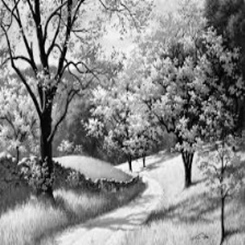
\includegraphics[width=4.57in,height=3.67in]{image5.png}
		\caption{Snapshot of working(Positive Sentiment)}
		\label{fig:Snapshot of working(Positive Sentiment)}
	\end{Center}
\end{figure}


%%%%%%%%%%%%%%%%%%%% Figure/Image No: 5 Ends here %%%%%%%%%%%%%%%%%%%%

\\
{\fontsize{11pt}{13.2pt}\selectfont \textbf{\textit{}}\par}
\end{Center}\par

\begin{Center}


%%%%%%%%%%%%%%%%%%%% Figure/Image No: 6 starts here %%%%%%%%%%%%%%%%%%%%

\begin{figure}[H]
	\begin{Center}
		\includegraphics[width=4.61in,height=3.81in]{image4.png}
		\caption{Snapshot of working(Negative Sentiment)}
		\label{fig:Snapshot of working(Negative Sentiment)}
	\end{Center}
\end{figure}


%%%%%%%%%%%%%%%%%%%% Figure/Image No: 6 Ends here %%%%%%%%%%%%%%%%%%%%

\\
\textbf{\textit{}}
\end{Center}\par


\vspace{\baselineskip}

\vspace{\baselineskip}
\section*{5\ \ \ \  CONCLUSION AND FUTURE ENHANCEMENT}
\addcontentsline{toc}{section}{5\ \ \ \  CONCLUSION AND FUTURE ENHANCEMENT}
\begin{justify}
We studied the tweets from twitter account of $``$GujaratTourism$"$. The lexicon-based approach was used to to build an extensive sentiment lexicon. The high precision subjectivity classifiers and polarity classifiers were used to generate the results. The overall accuracy that system was able to achieve was 63$\%$ . The system showed higher accuracy in classifying negative sentiments which was dropped while classifying positive sentiments. 
\end{justify}\par

\begin{justify}
As a future work, we have identified multiple works that can be carried out. Firstly, fine-grained level methods can be adopted to identify whether there is a polarity towards search term or not. Secondly, WSD methods can be implemented to increase the correctness of SentiWordNet analysis since WSD handles identification of word context problem. Thirdly, sarcasm detection can be applied as addressed in experiments and results section to improve the accuracy of results. Lastly, machine learning methods may be applied to understand the accuracy of them with respect to lexicon-based methods.
\end{justify}\par

\begin{justify}
 
\end{justify}\par


\vspace{\baselineskip}
\setlength{\parskip}{9.96pt}
\newpage
\begin{thebibliography}{99}

\vspace{\baselineskip}
\bibitem{item1}
Marrese-Taylor, E., Velasquez, J. D., $\&$  Bravo-Marquez, F. (2013). Opinion Zoom: A Modular Tool to Explore Tourism Opinions on the Web (pp. 261–264). IEEE. doi:10.1109/WI-IAT.2013.193\par

\bibitem{item2}
 W. Medhat, A. Hassan and H. Korashy, $``$Sentiment analysis algorithms and applications: A survey,$"$  Elsevier, Ain Shams Engineering Journal, vol. 5, Issue 4, pp. 1093-1113, December 2014.\par

\bibitem{item3}
R. Xia, F. Xu, C. Zong, Q. Li, Y. Qi, and T. Li, $``$Dual Sentiment Analysis: Considering Two Sides of One Review,$"$  IEEE Transactions on Knowledge and Data Engineering, vol. 27, Issue 8, pp. 2120-2133, August 2015.\par

\bibitem{item4}
A. El-Halees, $``$Mining opinions in user- generated contents to improve course evaluation,$"$  Software Engineering and Computer Systems, pp. 107-115, 2011.\par

\bibitem{item5}
Marrese-Taylor, E., Velasquez, J. D., $\&$  Bravo-Marquez, F. (2013). Opinion Zoom: A Modular Tool to Explore Tourism Opinions on the Web (pp. 261–264). IEEE. doi:10.1109/WI-IAT.2013.193\par

\setlength{\parskip}{12.0pt}
\bibitem{item6}
Colhon, M, Badica, C, $\&$  Sendre, A (2014). Relating the Opinion Holder and the Review Accuracy in Sentiment Analysis of Tourist Reviews. In Knowledge Science, Engineering and Management (pp.246-257). Springer International Publishing.\par

\bibitem{item7}
Himada, K., Inoue, S., $\&$  Endo, T (2012, September). On-site likelihood identification of tweets for tourism infonnation analysis. In Advanced Applied lnformatics (11A1AA1), 2012 IIAl International Conference on (pp. 117-122). IEEE.\par

\bibitem{item8}
H. Kaur, V. Mangat and Nidhi, "A survey of sentiment analysis techniques," ​ 2017 International Conference on I-SMAC (IoT in Social, Mobile, Analytics and Cloud) (I-SMAC) ​ , Palladam, 2017, pp. 921-925. Doi: 10.1109/I-SMAC.2017.8058315\par

\bibitem{item9}
B. K. Bhavitha, A. P. Rodrigues and N. N. Chiplunkar, "Comparative study of machine learning Techniques In sentimental analysis," 2017 International Conference On Inventive Communication and Computational Technologies (ICICCT), Coimbatore, 2017, pp. 216-221. Doi: 10.1109/ICICCT.2017.797\par

\bibitem{item10}
\href{https://www.safaribooksonline.com/library/view/natural-language-annotation/9781449332693/ch01.html}{https://www.safaribooksonline.com/library/view/natural-language-annotation/9781449332693/ch01.html}\par


\vspace{\baselineskip}
\setlength{\parskip}{9.96pt}

\end{thebibliography}

\vspace{\baselineskip}
\end{document}
